\documentclass{article}
\usepackage{geometry}[margin=1cm]
\usepackage{graphicx}
\usepackage{amssymb}
\begin{document}
{\bf Problem 1}

Triangle $ABC$ is inscribed in a circle $\Gamma$ with the centre at $O$, $|AB|=|CB|$. The segment $BB'$ is the diagonal of $\Gamma$. $O'$ is the midpoint of $OB'$. A circle $\Gamma'$ is drawn around $O'$ in such a way that the segment $AC$ is its chord. Prove that $\Gamma'$ intersects the segment $AB$ at its midpoint.
\begin{center}
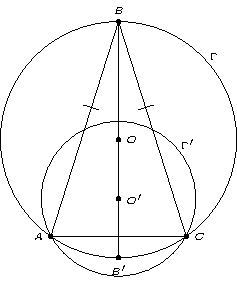
\includegraphics[width=0.5\textwidth]{Figures/fig1}
\end {center}

\end{document}
